\documentclass{sig-alternate-05-2015}

\usepackage{xcolor}
\usepackage{pifont}
\usepackage{paralist} % inparaenum support

\newcommand{\quadrat}{\ding{110}}%


\begin{document}
% No indent of paragraph
\parindent 0pt

% Copyright
\setcopyright{acmcopyright}
%\setcopyright{acmlicensed}
%\setcopyright{rightsretained}
%\setcopyright{usgov}
%\setcopyright{usgovmixed}
%\setcopyright{cagov}
%\setcopyright{cagovmixed}


% DOI
%\doi{10.475/123_4}

% ISBN
%\isbn{123-4567-24-567/08/06}

%Conference
\conferenceinfo{ACM SigSpatial '16}{October 31 - Thursday November 3, 2016, San
Francisco Bay Area, California, USA}

%\acmPrice{\$15.00}

%
% --- Author Metadata here ---
%\conferenceinfo{WOODSTOCK}{'97 El Paso, Texas USA}
%\CopyrightYear{2007} % Allows default copyright year (20XX) to be over-ridden
%- IF NEED BE.
%\crdata{0-12345-67-8/90/01}  % Allows default copyright data
%(0-89791-88-6/97/05) to be over-ridden - IF NEED BE.
% --- End of Author Metadata ---
%\title{BigGIS: A new generation predictive and prescriptive Geographic
%Information System}
\title{BigGIS: A Predictive and Prescriptive Geographic Information System
based on High-Dimensional Geo-Temporal Data Structures ("Vision Paper")}
%\titlenote{(Produces the permission block, and
%copyright information). For use with
%SIG-ALTERNATE.CLS. Supported by ACM.}}
%\subtitle{[Extended Abstract]
%\titlenote{A full version of this paper is available as
%\textit{Author's Guide to Preparing ACM SIG Proceedings Using
%\LaTeX$2_\epsilon$\ and BibTeX} at
%\texttt{www.acm.org/eaddress.htm}}}
%
% You need the command \numberofauthors to handle the 'placement
% and alignment' of the authors beneath the title.
%
% For aesthetic reasons, we recommend 'three authors at a time'
% i.e. three 'name/affiliation blocks' be placed beneath the title.
%
% NOTE: You are NOT restricted in how many 'rows' of
% "name/affiliations" may appear. We just ask that you restrict
% the number of 'columns' to three.
%
% Because of the available 'opening page real-estate'
% we ask you to refrain from putting more than six authors
% (two rows with three columns) beneath the article title.
% More than six makes the first-page appear very cluttered indeed.
%
% Use the \alignauthor commands to handle the names
% and affiliations for an 'aesthetic maximum' of six authors.
% Add names, affiliations, addresses for
% the seventh etc. author(s) as the argument for the
% \additionalauthors command.
% These 'additional authors' will be output/set for you
% without further effort on your part as the last section in
% the body of your article BEFORE References or any Appendices.

\numberofauthors{8} %  in this sample file, there are a *total*
% of EIGHT authors. SIX appear on the 'first-page' (for formatting
% reasons) and the remaining two appear in the \additionalauthors section.
%
\author{
% You can go ahead and credit any number of authors here,
% e.g. one 'row of three' or two rows (consisting of one row of three
% and a second row of one, two or three).
%
% The command \alignauthor (no curly braces needed) should
% precede each author name, affiliation/snail-mail address and
% e-mail address. Additionally, tag each line of
% affiliation/address with \affaddr, and tag the
% e-mail address with \email.
%
% 1st. author
%\titlenote{Maybe put address, e-mail here if allowed}
\alignauthor
Firstname Lastname\\
       \affaddr{University of Applied Sciences Karlsruhe}\\
%       \affaddr{Moltkestr. 30}\\
       \affaddr{Karlsruhe, Germany}\\
       \email{firstname.lastname@hs-karlsruhe.de}
% 2nd. author
\alignauthor
Firstname Lastname\\
       \affaddr{University of Applied Sciences Karlsruhe}\\
%       \affaddr{Moltkestr. 30}\\
       \affaddr{Karlsruhe, Germany}\\
       \email{firstname.lastname@hs-karlsruhe.de}
% 3rd. author
\alignauthor
Firstname Lastname\\
       \affaddr{FZI Research Center for Information Technology}\\
%       \affaddr{Haid-und-Neu-Str. 10-14}\\
       \affaddr{Karlsruhe, Germany}\\
       \email{lastname@fzi.de}
\and  % use '\and' if you need 'another row' of author names
%% 4th. author
\alignauthor
Firstname Lastname\\
       \affaddr{FZI Research Center for Information Technology}\\
%       \affaddr{Haid-und-Neu-Str. 10-14}\\
       \affaddr{Karlsruhe, Germany}\\
       \email{lastname@fzi.de}
%% 5th. author
\alignauthor
Firstname Lastname\\
%       \affaddr{Data Analysis and Visualization Group}\\
       \affaddr{University of Konstanz}\\
       \affaddr{Konstanz, Germany}\\
       \email{firstname.lastname@uni-konstanz.de}
%% 6th. author
\alignauthor
Firstname Lastname\\
%       \affaddr{Data Analysis and Visualization Group}\\
       \affaddr{University of Konstanz}\\
       \affaddr{Konstanz, Germany}\\
       \email{firstname.lastname@uni-konstanz.de}
}
% There's nothing stopping you putting the seventh, eighth, etc.
% author on the opening page (as the 'third row') but we ask,
% for aesthetic reasons that you place these 'additional authors'
% in the \additional authors block, viz.
\additionalauthors{\textcolor{red}{ToDO@all} John Smith (FZI,
email: {\texttt{jsmith@fzi.de}}), John Smith (Konstanz,
email: {\texttt{jsmith@konstanz.de}})}
%\date{30 July 1999}
% Just remember to make sure that the TOTAL number of authors
% is the number that will appear on the first page PLUS the
% number that will appear in the \additionalauthors section.

\maketitle
\begin{abstract}
Geographic information systems (GIS) are important tools for decision support
based on spatial data. Due to technical and economical progress an ever
increasing number of data sources are available leading to rapidly growing fast
and unreliable amount of data that can be beneficial 
\begin{inparaenum}[(1)]
	\item in the approximation of multivariate and causal predictions of future
values as well as
	\item in robust an proactive decision-making process. 
\end{inparaenum}
However, today's GIS are not designed for such demands and require new
methodologies to effectively model uncertainty and generate meaningful
knowledge. In this work, we introduce \textit{BigGIS}, a predictive and
prescriptive spatio-temporal analytics platform, that symbiotically
combines big data analytics, semantics and visual analytics methodologies. 
We introduce a novel continuous refinement model, present key elements and 
future challenges as we begin a collaborative research program into
methodologies for big data analysis and design for a big data enabled GIS.
\end{abstract}


%
% The code below should be generated by the tool at
% http://dl.acm.org/ccs.cfm
% Please copy and paste the code instead of the example below. 
%
%\begin{CCSXML}
%<ccs2012>
% <concept>
%  <concept_id>10010520.10010553.10010562</concept_id>
%  <concept_desc>Computer systems organization~Embedded systems</concept_desc>
%  <concept_significance>500</concept_significance>
% </concept>
% <concept>
%  <concept_id>10010520.10010575.10010755</concept_id>
%  <concept_desc>Computer systems organization~Redundancy</concept_desc>
%  <concept_significance>300</concept_significance>
% </concept>
% <concept>
%  <concept_id>10010520.10010553.10010554</concept_id>
%  <concept_desc>Computer systems organization~Robotics</concept_desc>
%  <concept_significance>100</concept_significance>
% </concept>
% <concept>
%  <concept_id>10003033.10003083.10003095</concept_id>
%  <concept_desc>Networks~Network reliability</concept_desc>
%  <concept_significance>100</concept_significance>
% </concept>
%</ccs2012>  
%\end{CCSXML}
%
%\ccsdesc[500]{Computer systems organization~Embedded systems}
%\ccsdesc[300]{Computer systems organization~Redundancy}
%\ccsdesc{Computer systems organization~Robotics}
%\ccsdesc[100]{Networks~Network reliability}


%
% End generated code
%

%
%  Use this command to print the description
%
%\printccsdesc

% We no longer use \terms command
%\terms{Theory}

\keywords{knowledge generation; big data analytics; data architecture}

\section{Introduction}
\label{sec:intro}
GIS have long been used to support the decision-making process
\cite{Crossland1995} in many
domains like civil planning, environment and nature protection or emergency
management. Thereby geospatial data have always been big data. Petabytes of
remotely sensed archival geodata (\textit{volume}) and a rapidly increasing
amount of real-time sensor data streams (\textit{velocity}) accelerate the need
for big data analytics in order to effectively model and efficiently process
complex geo-temporal problems. In the past, limited access to computing power
has been a bottleneck \cite{OGC2013}. However, in the era of cloud computing,
leveraging cloud-based resources is a widely adopted pattern (hardware level).
In addition, with the advent of big data analytics, performing massively
parallel analytical tasks on large-scale
data at rest or data in motion is as well becoming a feasible approach shaping
the design of today's GIS (software-level). Although scaling out enables GIS to
tackle the aforementioned big data induced requirements, there are still two
major open issues. Firstly, dealing with varying data types across multiple
data
sources (\textit{variety}) lead to data and schema heterogenity, e.g. to
describe locations, like addresses, relative spatial relationships or different
coordinates reference systems \cite{Frank.2016a}. Secondly, modelling the
inherent uncertainties in data (\textit{veracity}), e.g. real-world noise and
errorneous values due to the nature of the data collecting process. 
%\cite{Xiang2016}
Both being crucial tasks in data management and analytics
that
directly affect the information retrieval and decision-making quality and
moreover the generated knowledge on human-side (\textit{value}). Delegating
this
to only computed metrics often deprioritizes more important
macro
aspects of the problem. Current approaches mainly
address batch and stream analytics in their design oftentimes implemented as
a closed unified analytical GIS platform \cite{Thakur2015}. While the
importance
of such systems to efficiently deal with large amount of data is obvious,
computers miss the creativity of human analysis to create hidden connections
between data and problem domain \cite{SSS+14a}.

In this paper, we present the vision of \textit{BigGIS}, a new generation 
predictive and prescriptive GIS, that
leverages big data analytics, semantic reasoning and visual analytics
methodologies. This approach symbiotically combines system-side computation,
data storage and semantic reasoning capabilities with human-side perceptive
skills, cognitive reasoning and domain knowledge. We introduce a novel
\textit{continuous refinement model} to gradually minimize the real-world noise
and dissolve heterogenity in data and metadata such that the information gain
can be maximized. Our contribution lies in
\begin{inparaenum}[(1)]
  \item an \textit{integrated analytical pipeline approach} which includes
  \item \textit{semantic reasoning}, 
  \item \textit{human-related knowledge extraction and generation }as well as
  \item \textit{modelling uncertainty} to process
  high volume, high velocity and high dimensional spatio-temporal data from
  unreliable and heterogeneous sources.
\end{inparaenum}

Section \ref{sec:related} discusses related work and influencing research
fields. The platforms' design is introduced in Section \ref{sec:biggis}
through the continuous refinement model, while major challenges are
presented. Use cases are shown in Section \ref{sec:use}. Finally, Section
\ref{sec:concl} concludes and addresses future research topics.

\section{Related Work}
\label{sec:related}
Challenges related to the nature of big data has
lead to the evolution of new big data management and analytics architectures
embracing big data-aware GIS \cite{Peng2014}. Marz proposes the lambda
architecture \cite{Marz2013}, a generic, scalable and fault-tolerant data
processing system design. By decomposing the problem into three layers, namely
the batch layer, the speed layer, and the serving layer this architecture
hybridly combines batch analytics on historic data and stream analytics on
high-velocity streaming data to overcome eachs single weakenesses. Thakur et
al. introduces PlanetSense, a real-time streaming and spatio-temporal analytics
platform for gathering geo-spatial intelligence from open source data
\cite{Thakur2015}. Based on the lambda architecture, this platform enriches
large volumes of historic data by harvesting real-time data on the fly, e.g.
social media, or passive and participatory sensors. While this design allows
for adhoc analysis ability during batch runs,
the processing logic has to be implemented twice. In a more recent approach,
Kreps criticizes the overall complexity of the lambda architecture and presents
the kappa architecture~\cite{Kreps2014}, which simplifies the systems' design
by neglecting the batch layer. To replace batch processing,
static data is quickly fed through the streaming engine. An
interesting representative is Plasmap\footnote{\url{https://plasmap.io/}}, a
high performance geo-processing platform that provides a lightweight,
interactive query language for high-performance location discovery based on
OpenStreetMap. Developments in the field of semantic web services show the
opportunity of  adding  higher  semantic  levels  to existing frameworks,  to
improve
their  usage  and  ease  scalability, allowing for reasoning and comprehensive
responses~\cite{Tanasescu2006, Frank.2016a, Frank.2016b}.
Analyses are often performed in a descriptive, predictive or prescriptive 
way. While the descriptive analysis visualizes the status quo, predictive and 
prescriptive analysis focuses on future-oriented planning. As a result the 
underlying model and the visualization have to be tightly coupled in order for 
users to gain knowledge. Users have the possibility to interactively alter a 
model's parameters according to their knowledge, consequently the visualization
adjusts to the model in a feedback-loop. Knowledge generation is one important 
research area where visual analytics is of great
use~\cite{Keim2008, Keim2010}, especially
when considering uncertainty of heterogeneous spatio-temporal data from various
data sources \cite{SSK+16a}. J\"ackle et al. present one possible visualization
technique \cite{JSBK15} for data and uncertainties of large spatial datasets, 
which is crucial within use cases where both facets are of importance for
decision-making.
%Andrienko et al. states that geovisual analytics need new approaches to
%deal with the complexity of data and address a research agenda for
%working with spatio-temporal data \cite{Andrienko2010}.
% Plasmap differs from BigGIS in that domain expert knowledge is
%not used to train the system during runtime.

\section{BigGIS Platform}
\label{sec:biggis}

\subsection{Continuous Refinement Model in BigGIS}
\label{sec:crm}
In this section, we briefly describe the continuous refinement model in
BigGIS, which extends the knowledge generation model for visual
analytics \cite{SSS+14a}. This will on one hand allow to steadily
improve the analysis results e.g. by updating deployed machine learning models,
and on the other hand to build the user's trust in these results by creating
awareness of underlying uncertainties and data provenance which is key for
providing meaningful predictive and prescriptive decision support in various
fields \cite{SSK+16a}. We consider uncertainty to be reciprocally related to
generating new insights and consequently knowledge. Thus, modelling
uncertainty in BigGIS is a crucial  task. From a high-level perspective,
our approach consists of an integrated analytics 
pipeline which blends big data analytics and semantic reasoning on system-side
with knowledge extraction and generation on human-side, thereby modelling
uncertainty to continuously refine results as shown in Figure
\ref{fig:biggisworkflow}.
%\textcolor{red}{ToDO@all: Clearly define terms of \textit{user}, 
%\textit{semantics}, \textit{expert knowledge}, see issue \#16}


\begin{figure}
\centering
	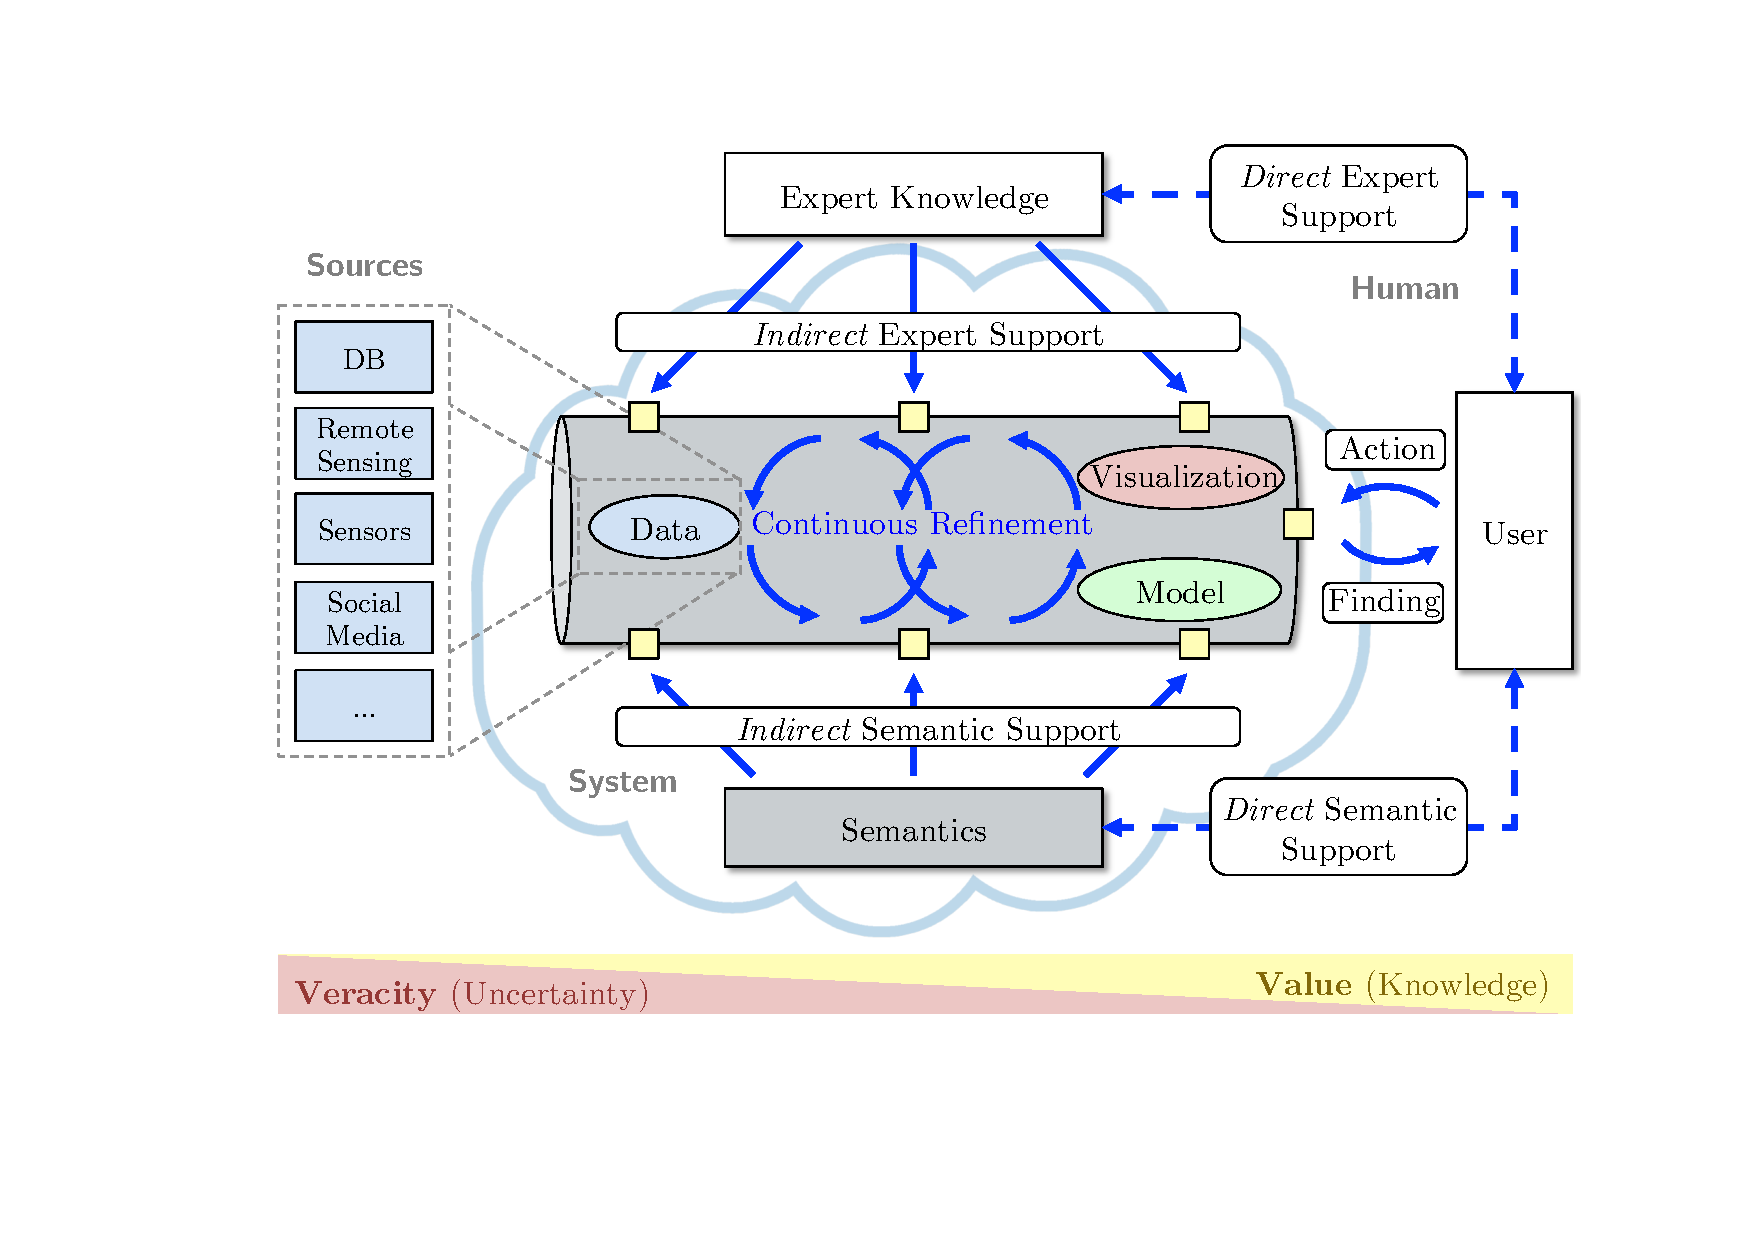
\includegraphics[width=\linewidth]{figures/biggis-workflow_v3}
	\caption{Continuous refinement model in BigGIS.}
	\label{fig:biggisworkflow}
\end{figure}

\subsubsection{Integrated Analytics Pipeline}
The analytics pipeline is the core of the continuous refinement model. A key 
abstraction within this model are specific access points called 
\textit{refinement gates} (see yellow squares in Figure 
\ref{fig:biggisworkflow}). Refinement gates allow for semantics and external 
expert knowledge to enter the pipeline at arbitrary stages during analyses to 
continuously improve data management and analytics results, e.g. to support
data 
preparation, to automatically deploy data transformation workflows, to provide 
expert domain knowledge in order to train machine learning models for pattern 
detection or to manipulate visualizations. 


\subsubsection{Semantic Reasoning}
Locating all available data sources that are relevant for meaningful findings
in analytical processes is hard to do when it has to be done manually. Semantic
web technology helps to describe data sources semantically using widely-applied 
vocabularies. Furthermore, semantic reasoning enables machines to discover 
suitable sources even if they are described differently, providing a two-level 
support for users through what we call \textit{linked APIs} and 
\textit{cognitive apps}. The former abstracts away the users from manually 
composing data integration workflows to unify heterogeneous data sources by 
using an appropriate ontology that supports the system (direct semantic 
support). The latter is a flexible service that is aware of a situational 
context and capable of sharing this with other services (indirect semantic 
support).

\subsubsection{Knowledge Extraction and Generation}
 The user is another relevant part in the continuous refinement model that is
either provided with additional expert knowledge by another person or he
himself is the expert in a specific field of application (direct expert
knowledge). Overall, we see the continuous refinement process as a knowledge
transfer from human (expert knowledge) to system which is reinforced by
semantic reasoning. Thereby, human knowledge is introduced to the system that
can contain additional domain specific information and constraints. By doing
so, big data analytics can 
\begin{inparaenum}[(1)]
 	\item leverage the creativity of human analysis to be able to establish
hidden connections between data and the problem domain and
	\item continuously refine the analyses quality and results.
\end{inparaenum}
The system intelligently learns from the provided external domain knowledge,
such that it can reuse it in the future (indirect expert support). Thus,
leading to an increasing likelihood of relevant findings by users during the
course of exploration and eventually to generating new knowledge.


\subsubsection{Modelling Uncertainty}
Uncertainty is inherent in data as well as models~\cite{cressie2015statistics}.
While this is often obvious in data like volunteered geographic information
and participatory sensed data, this holds true for all available data. The 
instruments employed by e.g. an official meteorological station have 
inaccuracies. Models derived from data are only perfectly applicable for the 
data upon which they are learned. Expert knowledge has some inherent 
uncertainty. To handle these uncertainties we express them as
\textit{conditional probabilities}. These conditional probabilities allow us
to evaluate and model the uncertainty of each data point as well as forecast of
an analytical model. We apply semantic reasoning on the provenance information
of data sources in order to infer a level of uncertainty that can be considered
in the analytical processes. We use \textit{bayesian hierarchical models} to be
able to cope with the conditional probabilities quantified by the semantic 
reasoning. The idea behind these models is that we can model the different 
parameters by their joint probability distribution. Each parameter can be model
by hyper-parameters, which are again probability distributions. The results 
models are then probability distributions as well, which can then be used in
our continuous refinement model. By doing so, we can model, examine and present
the uncertainty at each stage of the model to enable the user of BigGIS to make
a
well informed decision. 


\subsection{Challenges}
\label{sec:chls}
We identify three major challenges that are presented in the following.

\subsubsection{Varying big data related requirements}
Data volume and velocity are well-managed requirements through highly
scalable cloud-based big data architectures such as lambda architecture or
kappa architecture. Still, the field of application specifies the degrees of
big data related requirements. Thus, to provide a unified platform, efficiently
managing the complex backend ecosystem for varying requirements is a
non-trivial task. We approach this challenge by leveraging Apache
Mesos\footnote{\url{http://mesos.apache.org/}} in combination with
container technologies such as Docker \footnote{\url{https://www.docker.com/}}.
In addition, dealing with data and schema heterogenity and
inherent uncertainty is another interesting field of research that BigGIS
addresses.
Preconditions for meaningful findings in GIS are accurate, consistent
and complete data as input for analytical processes. However, sources of
spatio-temporal data are distributed and quality of the data is varying,
especially
when considering uncertain data like volunteered geographic information and
participatory sensing data. We address this challenge by a smart data
integration approach~\cite{Frank.2016a} which is based on semantically
described data sources and data transformation services. Smart web services
dynamically compose workflows of data sources and data transformation services
adopted to the requirements of different GISs based on the semantic meta
data~\cite{Frank.2016b}. 

\subsubsection{Dimensionality reduction}
The continuous refinement model employed in BigGIS is
dependent on a fast computation of possible data sources. The used data is
high-dimensional and models built upon this data can easily fall to the curse
of dimensionality. Also, while the presented architecture can handle the
challenges of big data, it is not always possible to transfer all the raw data
to our pipeline. In case of an automated sensor, e.g. on an unmanned aerial
vehicle, the transfer rate is dependent on the available bandwidth.
BigGIS aims to deal with the challenge of dimensionality reduction for
spatio-temporal data, balancing between the robustness of a model and the
adaptability to training and input data. 

\subsubsection{Bias-variance trade-off}
The bias-variance trade-off~\cite{Hastie2009} is of particular
interest in BigGIS, as the continuous refinement model as well as
the modelling of uncertainty are inherently connected to this.
Generally, solving this trade-off optimally is highly depending on the
specific use case. Providing the user with sufficient information to reason and
generate knowledge under these restrictions is one problem which we hope to
present a solution for. Here, the challenge lies in the speed of computation,
the different level of expertise for each user and the available bandwidth to
transfer informations back to the user and/or analytical pipeline.

\section{Use Cases}
\label{sec:use}
%\textcolor{red}{ToDO@all: please review and comment}
BigGIS will support decision-making in multiple use cases that require
processing of large and heterogeneous spatio-temporal data from unreliable
sources. The prototype will be evaluated on three scenarios: 
\begin{inparaenum}[(1)]
	\item smart city and health, i.e. heat stress in urban areas,
	\item environmental management, i.e. spread of invasive species,
	\item emergency management, i.e. identification and dispersion of hazardousgas in chemical accidents.
\end{inparaenum}
These scenarios represent diverse categories of application domains that each 
address varying big data related requirements. 
%In brief, one example is
%the environmental management scenario, where farmers can provide real-time
%data
%(velocity) from differing sources (variety), e.g. private weather stations,
%photos of invasive 
%species, or text messages about contaminated areas, though arriving with high 
%uncertainty (veracity). The experts domain knowledge helps to train
%classifiers
%in BigGIS on already available labeled datasets (volume) that, in addition to 
%further semantically described sources, helps conducting spatio-temporal 
%statistics such as hot spot analyses to make better predictions on potentially

%jeopardized areas. Not only are farmers informed about the condition of their 
%fields (descriptive) but also about risk potential of contamination 
%(predictive), which lastly results in suggestions to perform certain 
%counteractive measures (prescriptive).

%%this is just an alternative scenario; speech has to be updated.
In brief, an illustrating use case is supporting rescue forces in assessing
and managing large-scale and complex chemical disasters. Providing
an in-depth overview of the current situation within a small time frame
(velocity) is crucial to prevent exposing the surrounding population to any
hazardous substances. Recent developments in the field of
mobile robotics allow using in-situ components such as autonomously flying
unmanned aerial vehicles equipped with a hyperspectral camera that produces
several gigabyte of raw data per mission (volume). In addition, differing
sources (variety), e.g. private weather stations or social media streams, can
be integrated in BigGIS, though arriving with high uncertainty
(veracity). The combination of those datasets with various other
semantically described data sources, helps conducting spatio-temporal
statistics. Furthermore, the experts domain knowledge is used to train
classifiers in order to automatically classify the hazardous content and
identify contaminated areas. Conditional probabilities are computed to forecast
the dispersion of the hazardous smoke and visualized in risk-maps to highlight
potentially endangered areas. Not only are the rescue forces informed about the
current situation (descriptive), but also about risk potential of surrounding areas (predictive), which can be used to automatically alert further public
authorities and organizations that perform security tasks in
these areas (prescriptive).


\section{Conclusions and Future Work}
\label{sec:concl}
Big geo data is going to continue growing during the next years. The
rapidly increasing distribution and usage of mobile devices and IoT on the one
hand and emerging new data sources on the other hand lead to more diverse,
larger, faster and unreliable data. In this paper, we proposed BigGIS, a new
generation predictive and prescriptive GIS, that leverages big data analytics,
semantic reasoning and visual analytics methodologies through a novel
continuous refinement model, and showed what we consider are the key elements
to overcome uncertainty and generate meaningful knowledge. Therefore,
we identified three main challenges for the future. Currently, we are working
on a integrated prototype to support each of the presented use cases.

%\end{document}  % This is where a 'short' article might terminate

%ACKNOWLEDGMENTS are optional
\section{Acknowledgements}
\label{sec:ack}
This research has been funded by the Federal Ministry of Education and Research
of Germany (subsidy program IKT 2020 -- Forschung f\"ur Innovation).

%
% The following two commands are all you need in the
% initial runs of your .tex file to
% produce the bibliography for the citations in your paper.
\bibliographystyle{abbrv}
\bibliography{biggis-paper}  % sigproc.bib is the name of the
%Bibliography
%this case
% You must have a proper ".bib" file
%  and remember to run:
% latex bibtex latex latex
% to resolve all references
%
% ACM needs 'a single self-contained file'!
%
%APPENDICES are optional
%\balancecolumns
%\appendix
%Appendix A


\end{document}
